\documentclass[11pt, a4paper]{article}

\usepackage[utf8]{inputenc}
\usepackage[T1]{fontenc}
\usepackage[slovene]{babel}
\usepackage{lmodern}

\usepackage{xcolor}
\usepackage{bbold}
\usepackage{amsmath}
\usepackage{amssymb}
\usepackage{amsthm}

\usepackage{tikz}
% \usetikzlibrary{graphs,graphdrawing}

\usepackage{enumitem}
\setlist{nosep}
\renewcommand{\labelenumii}{\arabic{enumi}.\arabic{enumii}}

\setlength{\parindent}{0mm}

\usepackage{geometry}
\geometry{
    a4paper,
    left=5mm,
    right=5mm,
    top=5mm,
    bottom=15mm
}

% Standardne množice
\newcommand{\NN}{\mathbb{N}}
\newcommand{\ZZ}{\mathbb{Z}}
\newcommand{\QQ}{\mathbb{Q}}
\newcommand{\RR}{\mathbb{R}}
\newcommand{\CC}{\mathbb{C}}
\newcommand{\FF}{\mathbb{F}}

%%% Quantifiers
\newcommand{\all}[1]{\forall #1 \,.\,}
\newcommand{\some}[1]{\exists #1 \,.\,}
\newcommand{\exactlyone}[1]{\exists! #1 \,.\,}

% Implikacija
\newcommand{\lthen}{\Rightarrow}
\newcommand{\liff}{\Leftrightarrow}

%%% Množice
\newcommand{\set}[1]{\left\{#1\right\}}
\newcommand{\setb}[2]{\set{#1 \ | \  #2}}

%% Preslikave
\newcommand{\img}[1]{#1_{*}}
\newcommand{\invimg}[1]{#1^{*}}
\newcommand{\lin}[1]{\mathcal{#1}}

%% Odvod
\newcommand{\podv}[2]{\frac{\partial #1}{\partial #2}}

%% Metrični prostori
\newcommand{\norm}[1]{||#1||}

\DeclareMathOperator{\grad}{grad}




\begin{document}

\title{Diskretna matematika 1}
\maketitle

\section{Kombinatorika}
\subsection{Osnovna načela kombinatorike}
\begin{trditev}[Načelo produkta]
    Če sta $A, B$ končni množici, potem je $$|A \times B| = |A| \cdot |B|.$$
\end{trditev}

\begin{trditev}[Posplošeno načelo produkta]
    Če so $A_1, \ldots, A_k$ končne, potem je $$|\Pi_{i=1}^k A_i| = \Pi_{i=1}^k |A_i|.$$
\end{trditev}

\begin{trditev}[Načelo vsote]
    Če sta $A$ in $B$ končni in disjunktni množici, potem je $$|A \cup B| = |A| + |B|.$$
\end{trditev}

\begin{trditev}[Posplošeno načelo vsote]
    Če so $A_1, \ldots, A_k$ končne, paroma disjunktne množice, potem je $$\bigcup_{i=1}^k A_i = \sum_{i=1}^{k} |A_i|.$$
\end{trditev}

\begin{trditev}[Načelo enakosti]
    Če obstaja bijekcija $A \to B$, potem je $$|A|=|B|.$$
\end{trditev}

Označimo z $[k] = \set{1, 2, \ldots, k}$.

\begin{primer}
    Naj bo $A$ končna množica, $|A| = n$, $A = \set{a_1, a_2, \ldots, a_n}$. Naj bo $2^A$ potenčna množica. Določi moč $2^A$.
\end{primer}

\begin{trditev}[Načelo dvojnega preštevanja]
    Z njim pokažemo, da sta dva izraza/formuli enaka, če z obema na različna načina preštejemo elemente iste množice.
\end{trditev}

\begin{primer}[Eulorjeva funkcija $\phi$]
    Za $n \in \N$ definiramo $\phi(n) = \text{število števil iz } [n], \text{ ki so tuji z } n.$ Določi $\sum_{d | n} \phi(d)$.
\end{primer}

\begin{trditev}[Dirichletovo načelo]
    Če sta $n, m \in \N$ in je $n > m$, potem ne obstaja injektivna preslikava $[n] \to [m]$.
\end{trditev}

\begin{opomba}[Kombinatorična interpretacija]
    Če $n$ predmetov razporedimo v $m$ predalov in je $n > m$, potem sta vsaj v enem predalu vsaj dva predmeta.
\end{opomba}

\begin{primer}
    Naj bo $X \subset [100], \ |X|=10$. Pokaži, da $X$ vsebuje dve disjunktni podmnožici z isto vsoto.
\end{primer}

\subsection{Število preslikav}
\begin{definicija}
    Množica $B^A = \set{f: A \to B}$ je \emph{množica vseh preslikav iz $A$ v $B$}.
\end{definicija}

\begin{definicija} Definiramo:
    \begin{itemize}
        \item $n^{\underline{k}} = \underbrace{n(n-1) \ldots (n-k+1)}_\text{$k$ faktorjev}$ je \emph{padajoča potenca.}
        \item $n^{\overline{k}} = n(n+1) \ldots (n+k-1)$ je \emph{naraščajoča potenca.}
        \item $n! = ^{\underline{n}}$ je \emph{$n$ fakulteta}.
        \item Množica z $n$ elementi se imenuje \emph{$n$-množica.}
    \end{itemize}
\end{definicija}

\begin{trditev}
    Naj bosta $N$ in $K$ končni množici z $|N| = n, \ |K| = k$. Tedaj velja:
    \begin{enumerate}
        \item $|K^N| = k^n$.
        \item Število injektivnih preslikav iz $N$ v $K$ je $k^{\underline{n}}$.
        \item Število bijekcij iz $N$ v $K$ je $n!$, če $n = k$ in je $0$ sicer.
    \end{enumerate} 
\end{trditev}

\begin{proof}
    Za 1. in 2. točko uporabimo načelo enakosti. V 3. točki upoštevamo, kadar je preslikava iz končne množice v končno množico bijektivna.
\end{proof}

\newpage
\subsection{Binomski koeficienti in binomski izrek}
\begin{definicija}
    Naj bo $x \in \C$. Naj bo $k \in \N_0 = \set{1, 2, \ldots}$. Definiramo $\binom{x}{k} = \frac{x^{\underline{k}}}{k!} = \frac{x(x-1)\ldots (x-k+1)}{k!}$. 
    
    Števila $\binom{x}{k}$ so \emph{binomski koeficienti.}
    Če je $k \notin \N_0$ definiramo $\binom{x}{k} = 0$.
\end{definicija}

\begin{trditev}
    Če je $n \in \N_0$ in $k \leq n, \ k \in \N_0$, potem je 
    $$\binom{n}{k} = \frac{n!}{k!(n-k)!}.$$

    Števila $\binom{n}{k}$ so \emph{binomska števila.}
\end{trditev}

\begin{proof}
    Definicija binomskega koeficienta.
\end{proof}

\begin{opomba}
    Tudi $\binom{0}{0} = 1$. Razlaga: $0! = 1$ je število bijektivnih preslikav iz $\emptyset$ v $\emptyset$.
\end{opomba}

\begin{opomba}
    Če je $0 \leq k \leq n$, potem $\binom{n}{k} = \binom{n}{n-k}$.
\end{opomba}

\begin{definicija}
    Naj bo $N$ množica. Definiramo $\binom{N}{k} = \setb{A \in P(N)}{|A| = k}$.
\end{definicija}

\begin{trditev}
    Če je $N$ $n$-množica in je $0 \leq k \leq n$, potem je 
    $$\left| \binom{N}{k} \right| = \binom{n}{k}.$$
\end{trditev}

\begin{proof}
    Definiramo $X = \set{(n_1, n_2, \ldots, n_k); \ n_i \in \N \text{ paroma različni}}$. Označimo $X_{n,k} = \left| \binom{N}{k} \right|$. Preštejemo elementi množici $X$ na 2 načina.
\end{proof}

\begin{trditev}
    Za $n \in \N$ in $1 \leq k \leq n$ velja:
    $$\binom{n}{k} = \binom{n-1}{k-1} + \binom{n-1}{k}.$$
\end{trditev}

\begin{proof}
    Naj bo $N$ $n$-množica. Naj bo $x \in N$ poljuben fiksen element. 
    
    Definiramo $\mathcal{A} = \set{A \in \binom{N}{k}; \ x \in A}$ in $\mathcal{B} = \set{B \in \binom{N}{k}; \ x \notin B}$. Potem $\binom{N}{k} = \mathcal{A} \cup \mathcal{B}$. Uporabimo prejšnjo trditev in načelo vsote.
\end{proof}

\begin{definicija} 
    \emph{Pascalov trikotnik} je trikotnik oblike
    \[
    \setcounter{MaxMatrixCols}{20}   
    \begin{matrix}
        &&&&& 1 \\
        &&&& 1 && 1 \\
        &&& 1 && 2 && 1 \\
        && 1 && 3 && 3 && 1 \\
        & 1 && 4 && 6 && 4 && 1 \\
        1 && 5 && 10 && 10 && 5 && 1 

    \end{matrix}
    \]
\end{definicija}

\begin{opomba}
    S pomočjo Paskalovega trikotnika se lahko spomnimo rekurzivno formulo za $\binom{n}{k}$ ($n$ je številka vrstice, $k$ je številka diagonale, ki jo gledamo z leve proti desni). Šteteti vrstice in diagonale začnemo z $0$.
\end{opomba}

\begin{izrek}[Binomski izrek]
    Za vsak $n \in \N_0$ velja:
    $$(a+b)^n = \sum_{k=0}^{n} \binom{n}{k}a^kb^{n-k}.$$
\end{izrek}

\begin{proof}
    Izberimo $k$-krat $a$ izmed $n$ oklepajev.
\end{proof}

\begin{opomba}
    V izreku sta $a$ in $b$ elementi poljubnega komutativnega kolobarja.
\end{opomba}

\newpage
\subsection{Izbori}
Naj bo $N$ $n$-mnižica. Opazujemo izbori $k$-elementov.
\begin{enumerate}
    \item Izbor je urejen (važno v kakšnem vrstnem redu izberimo elementi):
    \begin{enumerate}
        \item Elementi si lahko ponavljajo: $n^k$.
        \item Elementi se ne smejo ponavljati: $n^{\underline{k}}$.
    \end{enumerate}
    \item Izbor je neurejen:
    \begin{enumerate}
        \item Elementi si lahko ponavljajo [trditev]: $\binom{n+k-1}{k}$.
        \item Elementi se ne smejo ponavljati: $\binom{n}{k}$.
    \end{enumerate}
\end{enumerate}

\begin{trditev}
    Število neurejenih izborov s ponavljanjem dolžine $k$ iz $n$-množice $N$ je 
    $$\binom{n+k-1}{k}.$$
\end{trditev}

\begin{proof}
    Naj bo $N = \set{x_1, x_2, \ldots, x_n}$. 
    
    Neurejenemu izboru $\underbrace{x_1\ldots x_1}_{k_1} \underbrace{x_2 \ldots x_2}_{k_2} \ldots \underbrace{x_n \ldots x_n}_{k_n}$ priredimo niz $\underbrace{1 \ldots 1}_{k_1} 0 \underbrace{1 \ldots 1}_{k_2} 0 \ldots 0 \underbrace{1 \ldots 1}_{k_n}$.
\end{proof}

\subsection{Permutacije in permutacije s ponavljanjem}
\begin{definicija}
    Naj bo $A$ $n$-množica. \emph{Permutacija množice $A$} je bijektivna preslikava $\pi: A \to A$.

    Množico vseh permutacij velikosti $n$ (permutacij na $[n]$) označimo z $S_n$. 
    Množico vseh permutacij množice $A$ označimo z $S_A$.
\end{definicija}

\begin{trditev}
    $|S_n| = n!$.
\end{trditev}

\begin{proof}
    Z indukcijo pokažemo, da je $|S_n| = n|S_{n-1}|$ in $|S_1| = 1$.
\end{proof}

\begin{trditev}
    Vsako permutacijo lahko zapišemo kot produkt disjunknih ciklov.
\end{trditev}

\begin{definicija}
    Naj bo $\pi \in S_n$. Par je \emph{inverzija}, če velja: $i < j$ in $\pi(i) > \pi(j)$.
\end{definicija}

\begin{definicija}
    Permutacija $\pi \in S_n$ je \emph{soda} (oz. \emph{liha}), če ima sodo mnogo inverzij (oz. liho mnogo inverzij).
\end{definicija}

\subsubsection{Multimnožice}
\begin{definicija}
    \emph{Multimnožica z elementi v množici $S$} je preslikava $\mu: S \to \N_0$. Pri tem številu $\mu(a), a \in S$, rečemo \emph{kratnost elementa $a$ v multimnožici $\mu$}, vsoti $\sum_{a \in S} \mu(a)$ pa \emph{moč multimnožice $\mu$}. Multimnožica je \emph{končna}, če je njena moč končna.
\end{definicija}

\begin{opomba}
    Multimnožico $M$ formalno podamo z urejenim parom $(S, \mu)$. Namesto da elemente zapišemo večkrat, lahko kratnost označimo tudi s formalno potenco: $M = \set{a, a, b, c, c, c} = \set{a^2, b, c^3}$.

    Multimnožica je isto kot neurejen izbor s ponavljanjem. Tojer obstaja $\binom{n+k-1}{k}$ $k$-elementnih multimnožic v množici z $n$ elementi.
\end{opomba}

\subsubsection{Permutacije multimnožic}
Permutacija multimnožice $M = (S, \mu)$ moči $n$ je zaporedje $(x_1, \ldots, x_n)$, kjer je $x_i \in S$ in se vsak $a \in S$ v zaporedju pojavi $\mu(a)$-krat.

\begin{trditev}
    Število permutacij multimnožice $M=\set{1^{\alpha_1}, 2^{\alpha_2}, \ldots, k^{\alpha_k}}$ moči $n = \alpha_1 + \ldots + \alpha_k$ je 
    $$\frac{n!}{\alpha_1!\alpha_2!\ldots\alpha_k!}.$$
\end{trditev}

\begin{proof}
    Najprej izberimo položaje elementa 1, nato izberimo položaje elementa 2 itd.
\end{proof}

\begin{definicija}
    Številu $\frac{n!}{\alpha_1! \alpha_2! \ldots \alpha_k!}$ rečemo \emph{multinomski koeficient} in ga označimo z $\binom{n}{\alpha_1, \alpha_2, \ldots, \alpha_k}$.
\end{definicija}

\begin{opomba}
    Multinomski koeficient je posplošitev binomskega koeficienta.
\end{opomba}

\begin{trditev}[Multinomski izrek]
    Velja 
    $$(x_1 + \ldots + x_k)^n = \sum \binom{n}{\alpha_1, \alpha_2, \ldots, \alpha_k}x_1^{\alpha_1} \ldots x_k^{\alpha_k},$$
    kjer vsota teče po vseh izbirah naravnih števil $\alpha_1, \ldots, \alpha_k$, katerih vsota je $n$.
\end{trditev}

\begin{proof}
    Število permutacij multimnožice moči $n$, kjer je $S$ množica indeksov.
\end{proof}

\subsection{Kompozicije naravnega števila}
\begin{definicija}
    \emph{Kompožicija naravnega števila $n$} je zaporedje pozitivnih naravnih števil $\lambda = (\lambda_1, \ldots, \lambda_l)$, za katero velja $\lambda_1 + \ldots + \lambda_l = n$. \emph{Dolžina} kompozicije $\lambda$, $l(\lambda)$ je število elemetnov zaporedja, številu $n$ pa rečemo \emph{velikost kompozicije}. Števila $\lambda_1, \ldots, \lambda_l$ imenujemo \emph{členi kompozicije}.
\end{definicija}

\begin{trditev}
    Naj bo $n \geq 1$.
    \begin{enumerate}
        \item Število kompožicij števila $n$ je enako $2^{n-1}$.
        \item Število kompožicij dolžine $k$ števila $n$ je enako $\binom{n-1}{k-1}$.
    \end{enumerate}
\end{trditev}

\begin{proof}
    Število $n$ lahko si predstavljamo kot zaporedje $n$ kgoglic, kompozicijo pa s pregradami med kroglicami: $\bullet~|~\bullet~\bullet~|~\bullet$.
\end{proof}

\begin{opomba}
    Lahko razumemo kompozicijo števila $n$ s $k$ členi kot rešitev enačbe $x_1 + \ldots + x_k = n$, kjer so $x_i \in \N$.
\end{opomba}

\subsubsection{Šibke kompozicije}
\emph{Šibka kompozicija števila $n$} ima isto definicijo kot kompozicija, le da dovolimo med členi tudi ničle.

\begin{trditev}
    Število šibkih kompozicij števila $n$ s $k$ členi je $\binom{n+k-1}{k-1} = \binom{n+k-1}{n}$.
\end{trditev}

\begin{proof}
    1. način. Rešujemo enačbo $x_1 + \ldots + x_k = n$, kjer so $x_i \in \N_0$.

    2. način. Kroglice in pregrade.

    3. način. Neurejeni izbori s ponavljanjem.
\end{proof}

\subsection{Razčlenitve naravnega števila}
\begin{definicija}
    \emph{Razčlenitev $n \in \N$} je zaporedje pozitivnih naravnih števil $\lambda = (\lambda_1, \ldots, \lambda_l)$, kjer je $\lambda_1 \geq \ldots \geq \lambda_l$ in $\lambda_1 + \ldots + \lambda_l = n$. \emph{Dolžina} razčlenitve $\lambda$, $l(\lambda)$ je število elementov zaporedja, številu $n$ pa rečemo \emph{velikost razčlenitve}. Števila $\lambda_1, \ldots, \lambda_l$ imenujemo \emph{členi razčlenitve}. Razčlenitvam rečemo tudi \emph{particije}.
\end{definicija}

\begin{definicija}
    Naj bo $\lambda = (\lambda_1, \ldots, \lambda_l)$ razčlenitev naravnega števila $n$. \emph{Ferrersov diagram $\lambda$} je seznam vrstic oblike:
    \begin{align*}
        \text{1. vrsta: } &\underbrace{\circ \ \circ \ \circ \ \ldots \ \circ}_{\lambda_1 \text{ krožcev}} \\
        \text{2. vrsta: } &\underbrace{\circ \ \circ \ \ldots \ \circ}_{\lambda_2 \text{ krožcev}} \\
        &\vdots \\
        \text{k. vrsta: } &\underbrace{\circ \ \ldots \ \circ}_{\lambda_l \text{ krožcev}}
    \end{align*}
\end{definicija}

\begin{definicija}
    Naj bo $\lambda = (\lambda_1, \ldots, \lambda_l)$ razčlenitev naravnega števila $n$. \emph{Konjugirana razčlenitev $\overline{\lambda}$} je razčlenitev, ki ima transponiran Ferrersov diagram.
\end{definicija}

Uvedemo oznake:
\begin{itemize}
    \item $p(n)$ je število razčlenitev števila $n$. Funkciji $p(n)$ rečemo tudi \emph{razčlenitvena funkcija}.
    \item $p_k(n)$ je število razčlenitev števila $n$ s $k$ členi.
    \item $\overline{p}_k(n)$ je število razčlenitev števila $n$ z največ $k$ členi.
\end{itemize}

\begin{trditev}
    Za naravni števili $n$ in $k$ velja:
    \begin{enumerate}
        \item $p_k(n) = p_{k-1}(n-1) + p_k(n-k)$.
        \item $p_k(n) = \overline{p}_k(n-k)$.
        \item $\overline{p}_k(n) = \overline{p}_{k-1}(n) + \overline{p}_k(n-k)$.
    \end{enumerate}
\end{trditev}

\begin{proof}
    Pomagamo si z Ferrersovim diagramom.
    \begin{enumerate}
        \item Razbijemo razčlinitve na tiste, ki vsebujejo $1$ in tiste, ki jo ne vsebujejo.
        \item Odštejemo od prvega stolpca $1$.
        \item Razčlenitev $n$ z največ $k$ členi ima bodisi natanko $k$ členov bodisi kvečjemi $k-1$ členov. \qedhere
    \end{enumerate}
\end{proof}

\subsection{Stirlingova števila I. vrste}
\begin{definicija}
    Naj bo $1 \leq k \leq n$. \emph{Stirlingovo število I. vrste $C(n,k)$} je število permutacij množice $[n]$, ki se zapišejo kot produkt $k$ disjunktnih ciklov.
    Velja: $C(n, 0) = 0, \ n > 0$ in $C(0,0) = 1$.
\end{definicija}

\begin{primer}
    Izračunaj $C(n,n), \ C(n, 1), \ C(4,2)$.
\end{primer}

\begin{trditev}
    Naj bo $1 \leq k \leq n$. Velja:
    $$C(n, k) = C(n-1, k-1) + (n-1)C(n-1, k).$$
\end{trditev}

\begin{proof}
    Permutacije $[n]$ s $k$ cikli razdelimo takole:
    \begin{enumerate}
        \item tiste, kjer je $n$ negibna točka in
        \item ostale. \qedhere
    \end{enumerate}
\end{proof}

Za izračun $C(n,k)$ lahko si pomagamo s Stirlingovo matriko I. vrste, ki jo dobimo s pomočjo rekurzivne zveze.

\begin{trditev}
    $x^{\overline{n}} = \sum_{k=0}^{\infty}C(n,k)x^k$.
\end{trditev}

\begin{proof}
    Indukcija po $n$.
\end{proof}

\begin{primer}
    Izračunaj $x^{\overline{4}}$.
\end{primer}

\subsection{Stirlingova števila II. vrste in Bellova števila}
\begin{definicija}
    \emph{Razdelitev množice $X$} je družina podmnožic $\set{X_i}_{i \in I}$ za katero velja:
    \begin{enumerate}
        \item $\bigcup_{i=I}X_i =X$,
        \item $X_i \cap X_j = \emptyset$ za vsaka $i,j \in I, \ i \neq j$.
    \end{enumerate}
\end{definicija}

\begin{definicija}
    Naj bo $1 \leq k \leq n$. \emph{Stirlingovo število II. vrste $S(n,k)$} je število razdelitev množice $[n]$ v $k$ nepraznih razredov. Velja: $S(n, 0) = 0, \ n > 0$ in $S(0,0) = 1$.
\end{definicija}

\begin{primer}
    Izračunaj $S(n, n), \ S(n, 1), \ S(n,2)$.
\end{primer}

\begin{definicija}
    \emph{Bellovo število $B(n) = \sum_{k=0}^{\infty} S(n,k)$} je število vseh razdelitev $n$-množice v neprazne razrede.
\end{definicija}

\begin{trditev}
    Naj bo $1 \leq k \leq n$. Velja:
    $$S(n,k) = S(n-1, k-1) + k S(n-1, k).$$
\end{trditev}

\begin{proof}
    Vzemimo množico $[n]$. Razdelitve v $k$ razredov razdelimo takole:
    \begin{enumerate}
        \item tiste, ki imajo $\set{n}$ kot samostojni del in
        \item ostale.
    \end{enumerate}
\end{proof}

Za izračun $S(n,k)$ lahko si pomagamo s Stirlingovo matriko II. vrste, ki jo dobimo s pomočjo rekurzivne zveze.

\begin{trditev}
    $x^n=\sum_{k=0}^{\infty} S(n,k) x^{\underline{k}}$.
\end{trditev}

\begin{proof}
    \textcolor{red}{TODO}
\end{proof}

\begin{opomba}
    Če dva polinoma stopnje $n$ ujemata v $n+1$ točk, potem sta enaka.
\end{opomba}

\begin{izrek}
    Število surjekcij iz $n$-množice v $k$-množico je enako 
    $$k! S(n,k).$$
\end{izrek}

\begin{proof}
    Vsaka surjekcija določa razdelitev $n$-množice v $k$ nepraznih razredov.
\end{proof}

\begin{trditev}
    $B(n+1) = \sum_{k=0}^{\infty} \binom{n}{k} B(k)$.
\end{trditev}

\begin{proof}
    \textcolor{red}{TODO}
\end{proof}

\begin{definicija}
    Naj bo $1 \leq k \leq n$. \emph{Lahovo število $L(n,k)$} je število razdelitev $n$-množice v $k$ linearno urejenih kosov.
\end{definicija}

\newpage
\subsection{Dvajnastera pot}
Naj bo $N$ $n$-množica (predmetov) in $K$ $k$-množica (predalov). 
Gledamo "`funkcijo"' $f: N \to K$, ki predmeti razporedi po predalih.

Imamo 12 možnosti: predmeti in predali lahko bodisi ločimo med seboj bodisi ne ločimo med seboj, funkcija lahko poljubna, inkjektivna (vsak predal ima kvečjemu 1 predmet) ali surjektivna (noben predal ni prazen).

\begin{izrek}[Dvajnastera pot]
    Velja:
    \begin{center}
        \begin{tabular}{ c | c | c | c }
            ločimo predmeti/predali & poljubna & injektivna  & surjektivna \\ 
            \hline
            DA/DA & $k^n$ & $k^{\underline{n}}$  & $k! S(n, k)$ \\ 
            \hline
            DA/NE & $\sum_{i \leq k} S(n, i)$ & $\begin{cases}
                1; &n \leq k \\
                0; &\text{sicer}
            \end{cases}$  & $S(n, k)$\\
            \hline 
            NE/DA & $\binom{n+k-1}{k-1}$ & $\begin{cases}
                \binom{k}{n}; &n \leq k \\
                0; &\text{sicer}
            \end{cases}$  & $\binom{n-1}{k-1}$ \\  
            \hline
            NE/NE & $\overline{p}_k(n)$ & $\begin{cases}
                1; &n \leq k \\
                0; &\text{sicer}
            \end{cases}$  & $p_k(n)$ 
        \end{tabular}
        \end{center}
\end{izrek}

\begin{proof}
    Uporabimo že znane rezultate (kompozicije, razčlenitve) itd.
\end{proof}

\subsection{Načelo vključitev in izključitev}
Recimo, da sta $A, B$ poljubni množici, potem $|A \cup B| = |A| + |B| - |A \cap B|$.
\begin{primer}
    Koliko so števil v $[30]$ ni tujih s $30$? Koliko so tujih?
\end{primer}

\begin{izrek}[Načelo vključitev in izključitev]
    Naj bo $A_1, \ldots, A_n$ množice. Velja: 
    $$\left| \bigcup_{i=1}^n A_i \right| = \sum_{j=1}^{n}(-1)^{j+1}\sigma_j,$$
    kjer je $\displaystyle \sigma_j = \sum_{I \in \binom{[n]}{j}} \left|\bigcap_{i \in I} A_i\right|$.
\end{izrek}

\begin{proof}
    Pokažemo, da če $x \in \bigcup_{i=1}^n A_i$, potem prispeva natanko $1$ k formuli.
\end{proof}

\begin{primer}
    Na koliko načinov lahko razporedimo $n$ označenih predmetov v $k$ označenih predalov, če je vsaj en predal prazen?
\end{primer}

\begin{posledica}
    Če je $X$ $N$-množica in so $A_1, \ldots, A_n \subset X$, potem je število elementov množice $X$, ki niso v nobeni izmed množic $A_1, \ldots, A_n$ enako 
    $$N + \sum_{j=1}^{n}(-1)^j \sigma_j.$$
\end{posledica}

\begin{definicija}
    \emph{Premestitev množice $[n]$} je permutacija $\pi \in S_n$ brez negibnih točk.
\end{definicija}

\begin{primer}
    Izračunaj število premestitev množice $[n]$.
\end{primer}

\begin{izrek}
    Če je $n = p_1^{e_1} \ldots p_r^{e^r}$ razcep $n \in \N$ na prafaktorji, potem je 
    $$\phi(n) = n(1 - \frac{a}{p_1}) \ldots (1 - \frac{1}{p_r}) \text{ (Eulorjeva funkcija)}.$$
\end{izrek}

\begin{proof}
    \textcolor{red}{TODO}
\end{proof}

\newpage
\subsection{Rekurzivne enačbe}
\begin{primer} 
    Na koliko načinov lahko prehodimo $n$ stopnic, če vsakič pregodimo $1$ ali $2$?
\end{primer}

\begin{primer}
    Koliko je dvojiških dreves s korenom z $n$ vozlišč?
\end{primer}

\begin{izrek}
    Naj bo zaporedje $(a_n)_{n \geq 0}$ podano takole:
    $$a_0 = b_0, \ a_1 = b_1, \ a_n = A a_{n-1} + B a_{n-2}, \ n \geq 2,$$
    kjer so $b_0, b_1, A, B$ fiksna števila. 
    Naj bosta $\alpha$ in $\beta$ korena \df{karakteristične enačbe} $x^2 = Ax + B$. Tedaj velja:
    \begin{enumerate}
        \item Če je $\alpha \neq \beta$, potem obstajata konstanti $K_1, K_2$, tako da je 
        $$a_n = K_1 \alpha^n + K_2 \beta^n.$$
        \item Če je $\alpha = \beta$, potem obstajata konstanti $K_1, K_2$, tako da je 
        $$a_n = (K_1 + K_2n) \alpha^n.$$     
    \end{enumerate}
\end{izrek}

\subsubsection*{Splošen primer}
Zaporedje $(a_n)_{n \geq 0}$ je podano takole:
\begin{enumerate}
    \item $a_0 = b_0, a_1 = b_1, \ldots, a_{d-1} = d _{d-1}$, kjer so $b_0, b_1, \ldots, b_{d-1}$ fiksna števila.
    \item $c_da_{n+d} + c_{d-1}a_{n+d-1} + \ldots + c_1 a _{n+1} + c_0 a_n = f(n) \ \textcolor{red}{(*)}$, kjer so $c_d, \ldots, c_0$ fiksna števila, $f(n): \N_0 \to \C$.
\end{enumerate}

\begin{definicija}
    \textcolor{red}{(*)} je \df{$d$-člena linearna rekurzija s konstantnimi koeficienti}. Če je $f(n) \equiv 0$, potem rečemo, da je rekurzija \textcolor{red}{(*)} \df{homogena}.
\end{definicija}

\subsubsection*{Kako rešemo homogeno rekurzijo?}
Zaporedja gledamo v prostoru $\C^{\N_0}$ vseh kompleksnih zaproedij. Naredimo vektorski prostor $(\C^{\N_0}, +, \cdot)$ na naraven način. Gledamo še prostor $\End(\C^{\N_0})$ in naredimo vektorski prostor $(\End(\C^{\N_0}), +, \circ)$.

Naj bo $E \in (\End(\C^{\N_0}))$, $E(a_0, a_1, a_2, \ldots) = (a_1, a_2, \ldots)$ (odrežemo prvi člen). BŠS: $c_d = 1$.
\begin{enumerate}
    \item Priredimo polinom: $Q(x) = x^d + c_{d-1}x^{d-1}+ \ldots + c_1x+c_0$.
    \item \textcolor{red}{\textbf{(!)}} Poglejmo $\ker Q(E)$:
    \begin{multline*}
        (a_n)_{n} \in \ker Q(E) \liff Q(E)((a_n)_n)= 0 \liff (E^d +c_{d-1}E^{d-1}+ \ldots + c_1 E +c_0 I)(a_n)_n = 0 \liff \\ \liff E^d(a_n)_n +c_{d-1}E^{d-1}(a_n)_n + \ldots +  c_1E(a_n)_n + c_0 I (a_n)_n = 0 \liff \\ \liff (a_d, a_{d+1}, \ldots) + c_{d-1}(a_{d-1}, a_d, \ldots) + \ldots + c_1(a_1, a_2, \ldots) + c_0 (a_0, a_1, \ldots) = 0 \liff \\ \liff (a_d +c_{d-1}a_{d-1} + \ldots + c_1a_1 + c_0a_0, \, a_{d+1}+c_{d-1}a_d + \ldots + c_1a_2 + c_0 a_1, \ldots) = 0 \liff (a_n)_n \text{ reši } \textcolor{red}{(*)}.
      \end{multline*}
      Torej splošne rešitve homogene enačbe so natanko elementi iz $\ker(Q(E))$.
      \item Polinom $Q(x)$ lahko zapišemo v obliki $Q(x) = (x-\lambda_1)^{s_1} \ldots (x-\lambda_k)^{s_k}$, potem       
      $$\ker Q(E) = \ker((E - \lambda_1I)^{s_1}) \oplus \ldots \oplus \ker((E - \lambda_kI)^{s_k}).$$
      Hočemo torej določiti $\ker ((E - \lambda I)^{s})$.
      \item Vemo: $\dim (\ker ((E - \lambda I)^{s})) = s$. Baza prostora je $(\lambda^n)_{n \geq 0}, (n\lambda^n)_{n \geq 0}, \ldots, (n^{s-1}\lambda^n)_{n \geq 0}$ (dokaz težek).
\end{enumerate}
\begin{izrek}
    $(a_n)_{n \geq 0} \in \ker ((E - \lambda I)^s) \liff a_n \text{ je oblike } a_n = P(n) \lambda^n$, kjer je $P(n)$ polinom stopnje kvečjemu $s-1$.
\end{izrek}

\begin{izrek}
    Splošna rešitev enačbe 
    $$c_da_{n+d} + c_{d-1}a_{n+d-1} + \ldots + c_1 a _{n+1} + c_0 a_n = 0$$
    je oblike 
    $$A_1(n) \lambda_1^n + \ldots + A_k(n) \lambda_k^n,$$
    kjer so $\lambda_i$ ničla karakterističnega polinoma kratnosti $s_i$, in je $A_i(n)$ polinom stopnje k večjemu $s_i - 1$ za vse $i \in [k]$.
\end{izrek}

\subsubsection*{Kako rešemo nehomogeno rekurzijo?}
Rešitev nehomogene enačbe 
$$c_da_{n+d} + c_{d-1}a_{n+d-1} + \ldots + c_1 a _{n+1} + c_0 a_n = f(n) \ \textcolor{red}{(*)}$$
je oblike 
$$z_n + b_n,$$
kjer je $z_n$ splošna rešitev ustrezne homogene enačbe in je $b_n$ neka partikularna rešitev enačbe \textcolor{red}{(*)}.

Pri tem $b_n$ praviloma iščemo z ustreznim nastavkom, pri čemer upoštevamo, da če je $f(n)$ aditivna, torej $$f(n)~=~f_1(n)~+~\ldots~+~f_t(n),$$ potem $b_n$ lahko dobimo kot vsoto partikularnih rešitev od $$c_da_{n+d} + c_{d-1}a_{n+d-1} + \ldots + c_1 a _{n+1} + c_0 a_n = f_i(n).$$

\begin{primer}
    Pri začetnih pogojah $a_0 = 0, \ a_1 = 1$, reši enačbo $a_n = 4a_{n-1} - 4a_{n-2} - 2n + 5 \cdot 3^n$.
\end{primer}

\subsection{Formalne potenčne vrste (Rodovne funkcije)}
\begin{definicija}
    Naj bo $a: \N \to \C$ zaporedje. Vrsta $\sum_{n \geq 0}a_n x^n$ je \df{formalna potenčna vrsta} zaporedja $a_n$.
\end{definicija}

\begin{definicija}
    Naj bo $(a_n)_n, \, (b_n)_n \in \C^{\N_0}$.
    \begin{itemize}
        \item $\sum_{n \geq 0}a_n x^n + \sum_{n \geq 0}b_n x^n = \sum_{n \geq 0}(a_n + b_n) x^n$.
        \item $\lambda \cdot \sum_{n \geq 0}a_n x^n = \sum_{n \geq 0}(\lambda a_n) x^n$.
        \item $(\sum_{n \geq 0}a_n x^n) \cdot (\sum_{n \geq 0}b_n x^n) = \sum_{n \geq 0}c_n x^n$, kjer $c_n = \sum_{k=0}^{n}a_kb_{n-k}$.
    \end{itemize}
\end{definicija}

\begin{opomba}
    Formalne potenčne vrste tvorijo algebro.
\end{opomba}

\begin{definicija}
    F.\ p.\ v.\ $A(x)$ je \df{obrnljiva}, če obstaja f.\ p.\ v.\ $B(x)$, da velja $A(x) \cdot B(x) = (1, 0, 0, \ldots)$.
\end{definicija}

\begin{trditev}
    Formalna potenčna vrsta $A(x)$ je obrnljiva natanko tedaj, ko $a_0 \neq 0$
\end{trditev}

\begin{proof}
    $(\lthen)$ Definicija množenja.

    $(\Leftarrow)$ Induktivno konstruiramo členi f.\ p.\ v.\ $B(x)$.
\end{proof}

\begin{definicija}
    Če je $(a_n)_n$ zaporedje, ki je rešitev nekega kombinatoričnega problema, potem $\sum_{n \geq 0}a_n x^n$ pravimo \df{rodovna funkcija}. Pišemo: $G(x) = \sum_{n \geq 0}a_n x^n$.
\end{definicija}

\begin{primer}
    Določi rodovno funkcijio Fibonaccijeva zaporedja.
\end{primer}

\begin{definicija}
    Naj bo $A(x) = \sum_{n \geq 0}a_n x^n$ f.\ p.\ v. \df{Odvod} f.\ p.\ v.\ je $A'(x) =  \sum_{n \geq 1}na_n x^{n-1} =  \sum_{n \geq 0}(n+1)a_n x^n$.
\end{definicija}

\begin{trditev}
    $(A(x) \cdot B(x))' = A'(x)B(x) + A(x)B'(x)$.
\end{trditev}

\begin{proof}
    Račun.
\end{proof}

\subsubsection*{Reševanje rekurzij z rodovnimi funkcijami}
\begin{primer}
    Naj bo $a_0 = 2, a_1 = 3, a_n = 2a_{n-1}-a_{n-2}, n \geq 2$. Določi splošno formulo za $a_n$.
\end{primer}
\paragraph{Koraki splošnega reševanja nekega kombinatoričnega problema}
\begin{enumerate}
    \item Rešitev problema zapišemo z rekurzivno enačbo.
    \item Zapišemo rodovno funkcijio zaporedja z pomočjo rekurzivne zveze.
    \item Z algebro nad rodovnimi funkcijami, rodovno funkcijo razvijemo v vrsto.
    \item Iz razvoja preberemo rešitev našega začetnega problema.
\end{enumerate}

\subsection{Catalanova števila}
Imejmo produkt $n$ števil $x_1x_2 \ldots x_n$. Na koliko načinov lahko izračunamo ta produkt, če po vrsti zmnožimo dve zaporedni števili in jih nadomestimo s produktom?

\begin{definicija}
    \df{Catalanovo število $C_n$} je število načinov, s katerimi lahko izračunamo produkt $x_1x_2 \ldots x_n$.
\end{definicija}

\begin{opomba}
    Velja rekurzivna zveza: $a_n = \sum_{k=0}^{n-1}a_ka_{n-k-1}$.
\end{opomba}

\begin{trditev}
    $C_n = \frac{1}{n+1} \binom{2n}{n}$.
\end{trditev}

\begin{proof}
    Rodovne funkcije.
\end{proof}


\newpage
\section{Teorija grafov}
\subsection{Osnovni pojmi}
\begin{definicija}
    \emph{Graf} G je urejen par $(V(G), E(G))$, kjer je $V(G)$ množica \emph{vozlišč} grafa $G$ in $E(G)$ množica \emph{povezav} grafa~$G$, kjer je $E(G) \subseteq \binom{V(G)}{2}$.
\end{definicija}

\begin{opomba}
    Če ne povemo drugače, bo množica $V(G)$ končna.
\end{opomba}

\begin{opomba}
    Naj bo $\set{u, v} \in E(G)$:
    \begin{itemize}
        \item Krajše pišemo $uv$.
        \item Pravimo, da sta $u$ in $v$ \emph{krajišči} povezave $e$ in, da sta $u$ in $v$ \emph{sosedni} vozlišči.        
        Pišemo: $u \sim v$ ali $u \sim_G v$.
    \end{itemize}
\end{opomba}

\begin{definicija}
    Naj bo $G$ graf, $u \in V(G)$:
    \begin{itemize}
        \item $N_G(u) = \setb{v \in V(G)}{uv \in E(G)}$ je \emph{soseščina} vozlišča $u$.
        \item $\deg_G(u) = |N_G(u)|$ je \emph{stopnja} vozlišča $u$. Označimo z $\delta(G) = \min_{v \in V(G)}\deg_G(v)$.
    \end{itemize}
\end{definicija}

\begin{definicija}
    Graf $G$ je \emph{regularen}, če imajo vsa vozlišča isto stopnjo.
\end{definicija}

\begin{opomba}
    Če je ta stopnja $r$, pravimo, da je $G$ $r$-regularen graf.
\end{opomba}

\begin{primer}
    Petersenov graf $P$ je $3$-regularen graf:
    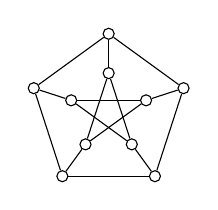
\begin{tikzpicture}[scale=1, auto, node distance=2cm]

        % Вершины внешнего цикла
        \node[circle, draw, minimum size=4pt, inner sep=0pt] (A) at (90:1) {};
        \node[circle, draw, minimum size=4pt, inner sep=0pt] (B) at (162:1) {};
        \node[circle, draw, minimum size=4pt, inner sep=0pt] (C) at (234:1) {};
        \node[circle, draw, minimum size=4pt, inner sep=0pt] (D) at (306:1) {};
        \node[circle, draw, minimum size=4pt, inner sep=0pt] (E) at (18:1) {};
        
        % Вершины внутреннего звёздного графа
        \node[circle, draw, minimum size=4pt, inner sep=0pt] (A1) at (90:0.5) {};
        \node[circle, draw, minimum size=4pt, inner sep=0pt] (B1) at (162:0.5) {};
        \node[circle, draw, minimum size=4pt, inner sep=0pt] (C1) at (234:0.5) {};
        \node[circle, draw, minimum size=4pt, inner sep=0pt] (D1) at (306:0.5) {};
        \node[circle, draw, minimum size=4pt, inner sep=0pt] (E1) at (18:0.5) {};
        
        % Рёбра внешнего цикла
        \draw (A) -- (B);
        \draw (B) -- (C);
        \draw (C) -- (D);
        \draw (D) -- (E);
        \draw (E) -- (A);
        
        % Рёбра внутреннего цикла (звезды)
        \draw (A1) -- (C1);
        \draw (C1) -- (E1);
        \draw (E1) -- (B1);
        \draw (B1) -- (D1);
        \draw (D1) -- (A1);
        
        % Соединения внешнего и внутреннего циклов
        \draw (A) -- (A1);
        \draw (B) -- (B1);
        \draw (C) -- (C1);
        \draw (D) -- (D1);
        \draw (E) -- (E1);
    
    \end{tikzpicture}
\end{primer}

\begin{primer}
    Grafe lahko predstavimo tudi z matrikami. Možnosti:
    \begin{enumerate}
        \item \emph{Matrika sosednosti.} Za graf $G$ z vozlišči $v_1, \ldots, v_n$ je matrika sosednosti matrika $A(G) \in \R^{n \times n}$, definirana z $$a_{ij} = \begin{cases}
            1, &v_i \sim v_j, \\
            0, &v_i \nsim v_j.
        \end{cases}.$$
        \item \emph{Incidenčna matrika}. Če ima graf $G$  vozlišča $v_1, \ldots, v_n$ in povezave $e_1, \ldots, e_m$, je to matrika $B(G) \in \R^{n \times m}$, podana s predpisom $$b_{ij} = \begin{cases}
            1, &v_i \in e_j, \\
            0, &v_i \notin e_j.
        \end{cases}.$$
    \end{enumerate}
\end{primer}

\subsection{Lema o rokovanju}
\begin{lema}[o rokovanju]
    Naj bo $G$ graf. Velja: $$\sum_{u \in V(G)} \deg_G(u) = 2 \cdot |E(G)|.$$
\end{lema}

\begin{proof}
    Incidenčna matrika in načelo dvojnega preštevanja.
\end{proof}

\begin{posledica}
    Število vozlišč lihe stopnje danega grafa je sodo.
\end{posledica}

\begin{proof}
    Razbijemo vsoto na vozlišče sode in lihe stopnje.
\end{proof}

\subsection{Podgrafi}
\begin{definicija}
    Naj bosta $G$ in $H$ grafa. Če velja $V(H) \subseteq V(G)$ in $E(H) \subseteq E(G)$, tedaj rečemo, da je $H$ \emph{podgraf} grafa~$G$, in pišemo $H \leq G$. Pri tem:
    \begin{itemize}
        \item Podgraf $H$ je \emph{vpet} podgraf, če je $V(H) = V(G)$ (odstranimo nekaj povezav).
        \item Podgraf $H$ je \emph{porojen} (oz. \emph{induciran}), če velja:  $\all{u, v \in V(H)} u \sim_G v \lthen u \sim_H v$ (odstranimo nekaj vozlišč).
    \end{itemize}
\end{definicija}

\newpage
\subsection{Nekatere družine grafov}
\paragraph{Polni grafi.} Naj bo $V$ poljubna neprazna množica. Tedaj grafu z množico vozlišč $V$ in množico povezav $\binom{V}{2}$ vseh neurejenih parov elementov iz $V$ rečemo \emph{polni graf} z množico vozlišč $V$. Oznaka: $K_V$ ali $K_n$, če $V = [n]$.

\paragraph{Poti.} Grafu z množico vozlišč $\Z_n$ in množico povezav $E(P_n) = \setb{i(i+1)}{i \in \set{0,1, \ldots, n-2}}$ rečemo \emph{pot dolžine~$n$}. Oznaka: $P_n$.

\paragraph{Cikli.} Za $n \in \N, n \geq 3$, s $C_n$ označimo graf z množico vozlišč $\Z_n$ in množico povezav $E(C_n) = \setb{i(i+1)}{i \in \Z_n}$. Grafu $C_n$ rečemo \emph{cikel dolžine $n$}.

\paragraph{Polni dvodelni grafi.} Naj bosta $A$ in $B$ poljubni disjunktni neprazni množici. Grafu $K_{A, B}$ z množico vozlišč $A \cup B$ in množico povezav $E(K_{A,B}) = \setb{uv}{u \in A, v \in B}$ rečemo \emph{polni dvodelni graf} na paru množic $A, B$. Oznaka: $K_{A, B}$ ali $K_{m, n}$, če $A = [m], \ B = [n]$.

\paragraph{Hiperkocke.} Za $d \in \N$ naj $\Z_2^d$ predstavlja množico vseh urejenih $d$-teric ničel in enic. Na $\Z_2^d$ lahko gledamo kot na Abelovo grupo. Za $i \in {1, 2, \ldots, d}$ naj bo $e_i$ tisti element množice $\Z_2^d$, ki ima na $i$-tem mestu enico, povsod drugod pa ničlo. Pišimo $S = \set{e_1, e_2, \ldots, e_d}$. \emph{Hiperkocka razsežnosti $d$} je graf z množico vozlišč $\Z_2^d$ in z dvema vozliščema $u, v \in \Z_2^d$ sosednjima, če in samo če je $u+ v \in S$, tj. $u$ in $v$ razlikujeta v natanko eni komponenti. Oznaka: $Q_n$. Velja:
\begin{itemize}
    \item $|V(Q_n)| = 2^d$.
    \item $|E(Q_n)| = d \cdot 2 ^{d-1}$.
\end{itemize}

\paragraph{Posplošeni Petersenovi grafi.} Naj bosta $n, k \in \N, \ n \geq 3, \ 2k < n$. Naj bosta $U = \set{u_0, u_1, \ldots, u_{n-1}}$ in $V~=~\set{v_0, v_1, \ldots, v_{n-1}}$ dve disjunktni $n$-elementni množici. \emph{Posplošeni Petersonov graf $P_{n,k}$} je graf z množico vozlišč $V(P_{n,k}) = U \cup V$ in množico povezav enako $E(P_{n,k}) = E_1 \cup E_2 \cup E_3$, kjer je 
$$E_1 = \setb{u_iu_{i+1}}{i \in \Z_n}, \quad E_2 = \setb{v_iv_{i+k}}{i \in Z_n}, \quad E_3 = \setb{u_iv_i}{i \in \Z_n}.$$

\subsection{Sprehodi, poti in cikli}
\begin{definicija}
    \emph{Sprehod} v grafu $G$ je zaporedje vozlišč grafa $G$: $v_0v_1\ldots v_k$, tako da je $v_iv_{i+1} \in E(G)$ za $i \in [k-1]$. Rečemo, da je to $v_0v_k$-sprehod. Sprehod je \emph{enostaven}, če so vse njegove povezave paroma različne.
\end{definicija}

\begin{definicija}
    \emph{Pot} v grafu $G$ je sprehod s samimi različnimi vozlišči.
\end{definicija}

\begin{definicija}
    Če ima sprehod v grafu $G$ isti začetek in konec pravimo, da je sprehod \emph{sklenjen}. \emph{Enostaven sklenjen sprehod} je sklenjen sprehod, ki je enostaven. \emph{Cikel} v grafu $G$ je sklenjen sprehod z samimi različnimi vozlišči.
\end{definicija}

\begin{lema}
    Če v grafu $G$ obstaja $uv$-sprehod, obstaja tudi $uv$-pot.
\end{lema}

\begin{proof}
    Cilj: paroma različna vozlišča.
\end{proof}

\begin{lema}
    Če v grafu $G$ obstajata dve različi $uv$-poti, potem ima $G$ vsaj en cikel.
\end{lema}

\begin{proof}
    Skupna vozlišča.
\end{proof}

\begin{lema}
    Če v grafu $G$ obstaja sklenjen sprehod lihe dolžine, obstaja v $G$ tudi cikel lihe dolžine.
\end{lema}

\begin{proof}
    Indukcija na dolžino sprehoda.
\end{proof}

\subsection{Povezane komponente, razdalja in premer}
\begin{definicija}
    Graf $G$ je \emph{povezan}, če za vsak par vozlišč $u, v \in V(G)$ obstaja $uv$-sprehod (ekvivalentno: $uv$-pot).
\end{definicija}

\begin{definicija}
    Maksimalni podgrafi grafa, ki so povezani, so \emph{komponente} grafa. 
\end{definicija}
Označimo z $\Omega(G)$ število komponent grafa $G$.

\begin{definicija}
    Naj bo $G$ povezan graf, $u, v \in V(G)$. \emph{Razdalja $d_G(u,v)$} med $u$ in $v$ je število povezav na najkrajši $uv$-poti.
\end{definicija}

\begin{opomba}
    Naj bo $G$ povezan graf. Velja:
    \begin{itemize}
        \item $d_G(u,v) = 0 \liff u = v$.
        \item $d_G(u,v) = 1 \liff uv \in E(G)$.
    \end{itemize}
\end{opomba}

\begin{trditev}
    Naj bo $G$ povezan graf. Potem $(V(G), d_G)$ je metrični prostor.
\end{trditev}

\begin{proof}
    Preverimo lastnosti.
\end{proof}

\newpage
\begin{definicija}
    Naj bo $G$ povezan graf. \emph{Ekscentričnost $\ecc_G(u)$} vozlišča $u$ je $\max_{v \in V(G)} d_g(u,v)$.
\end{definicija}

\begin{definicija}
    Naj bo $G$ povezan graf. \emph{Premer $\diam G$} grafa $G$ je $\max_{u \in V(G)} \ecc_G(u) = \max_{u,v \in V(G)} d_G(u,v)$.
\end{definicija}

\begin{definicija}
    Naj bo $G$ povezan graf. \emph{Polmer $\rad(G)$} grafa $G$ je $\min_{u \in V(G)} \ecc_G(u)$
\end{definicija}

\begin{primer}
    Velja:
    \begin{itemize}
        \item $\diam(P_{5,2}) = \rad(P_{5,2}) = 2$.
        \item $\diam(P_n) = n-1, \ \rad(P_n) = \lfloor \frac{n}{2} \rfloor$.
    \end{itemize} 
\end{primer}

\subsection{Inačice koncepta "`graf"'}
\paragraph{Enostavni grafi.} Lahko dopuščamo \emph{vzporedne povezave}, tj. množica povezav lahko multimnožica, in \emph{zanke}, tj. povezave iz vozlišča vase.
\begin{definicija}
    Graf je \emph{enostaven}, če nima vzporednih povezav in zank.
\end{definicija}

\paragraph{Uteženi grafi, omrežja.} Lahko definiramo:
\begin{itemize}
    \item $G = (V(G), E(G), w)$, kjer je $w: V(G) \to \R$ je \emph{uteženi} graf.
    \item $G = (V(G), E(G), l)$, kjer je $l: E(G) \to \R$ je \emph{omrežje}.
    \item $G = (V(G), E(G), w, l)$, je \emph{uteženo omrežje}. 
\end{itemize}

\paragraph{Usmerjeni grafi.} Množica povezav $E(G)$ grafa $G$ lahko podmnožica $V(G) \times V(G)$, tj. povezave so urejeni pari.

\paragraph{Hipergrafi.} Elementi $E(G)$ so lahko množice poljubne kardinalnosti.

\subsection{Dvodelnost}
\begin{definicija}
    Graf $G$ je \emph{dvodelen}, če obstaja razdelitev $V(G) = V_1 \cup V_2$, tako da velja: $$uv \in E(G) \lthen u \in V_1 \land v \in V_2.$$
\end{definicija}

\begin{opomba}
    Dvodelnost grafa lahko raziščemo z barvanjo vozlišč z dvema barvama.
\end{opomba}

\begin{izrek}
    Graf $G$ je dvodelen natanko tedaj, ko ne vsebuje lihih ciklov.
\end{izrek}

\begin{proof}
    $(\lthen)$ Imamo težavo z barvanjo cikla.
    
    $(\Leftarrow)$ Izberimo $x \in V(G)$ in razdelimo $V(G)$ na vozlišča, ki so na sode razdalje od $x$ in, ki so na lihe razdalje od $x$. Pokažemo, da znotraj posameznih množic ni povezav.
\end{proof}

\subsection{Morfizmi grafov}
\subsubsection*{Homomorfizmi grafov}
\begin{definicija}
    Naj bosta $G, H$ grafa. Preslikava $f: V(G) \to V(H)$ je \emph{homomorfizem}, če velja: $$uv \in E(G) \lthen f(u)f(v) \in E(H).$$
    Injektivni homomorfizem je \emph{vložitev} grafa $G$ v graf $H$.
\end{definicija}

\begin{opomba}
    Če je $G$ dvodelen, potem obstaja homomorfizem $f: G \to K_2$.
\end{opomba}

\begin{definicija}
    Vložitev $f: V(G) \to V(H)$ grafa $G$ v graf $H$ je \emph{izometrična}, če velja:
    $$\all{u, v \in V(G)}d_G(u,v)=d_H(f(u), f(v)).$$
\end{definicija}

\begin{primer}
    Preslikava $\varphi: V(C_4) \to V(Q_3)$ definarana s 
    \begin{center}
        \begin{tabular}{ c | c c c c }
         $x$ & 0 & 1 & 2 & 3 \\ \hline
         $\varphi(x)$ & 000 & 100 & 110 & 010  
        \end{tabular}
    \end{center}
    je homomorfizem.
\end{primer}

\subsubsection*{Izomorfizmi grafov}
\begin{definicija}
    Naj bosta $G, H$ grafa. Preslikava $f: V(G) \to V(H)$ je \emph{izomorfizem}, če
    \begin{enumerate}
        \item $f$ je bijekcija;
        \item $f$ je homomorfizem;
        \item $f^{-1}$ je homomorfizem.
    \end{enumerate}
\end{definicija}

\begin{opomba}
    Pogoj 2. pravi, da $f$ slika povezave v povezave. Pogoj 3. pravi, da $f$ slika nepovezave v nepovezave.
\end{opomba}

\begin{definicija}
    Grafa $G$ in $H$ sta \emph{izomorfna}, če obstaja izomorfizem med njima. Oznaka: $G \cong H$.
\end{definicija}

\begin{opomba}
    Izomorfnost je ekvivalenčna relacija.
\end{opomba}

\begin{primer}
    Dokaži, da $Q_3 \cong K_{4,4}$
\end{primer}

\begin{opomba}
    Izomorfnost je algoritmično zahtevna naloga. Če za dva grafa domnevamo, da sta izomorfna, potem to dokažemo tako, da med njima poiščemo izomorfizem. Če za dva grafa domnevamo, da nista izomorfna, tedaj to najlažje dokažemo tako, da poiščemo neko številsko karakteristiko grafov, v kateri se razlikujeta, pri izomorfizmu pa se ohranja: število vozlišč, število povezav, ožina, število podgrafov izbrane vrste (trikotniki, cikli dolžine 4), urejeno zaporedje snopenj vozlišč. Lahko si pomagamo z lastnosti grafov: povezanost, dvodelnost.
\end{opomba}

\subsubsection*{Grupa avtomorfizmov grafa}
\begin{definicija}
    \emph{Avtomorfizem} grafa $G$ je izomorfizem $f: G \to G$.
\end{definicija}

Definiramo $\Aut (G) = \setb{\varphi}{\varphi \text{ je avtomorfizem grafa } G}$. Dodamo še komponiranje in dobimo \emph{grupo avtomorfizmov grafa $G$}.

\begin{opomba}
    Velja:
    \begin{itemize}
        \item Vsaka končna grupa je grupa avtomorfizmov nekega grafa.
        \item $\Aut(K_n) \cong S_n$, $\Aut(P_n) \cong \Z_2$, $\Aut(C_n) \cong D_{2n}$.
        \item Skoraj vsi grafi imajo trivialno grupo $\Aut(G)$.
    \end{itemize}
\end{opomba}

\subsection{Operacije z grafi}
\subsubsection*{Komplementarni graf}
\begin{definicija}
    \emph{Komplement $\overline{G}$} grafa $G$ je graf z isto množico vozlišč kot $G$ in z dvema vozliščema sosednjima v $\overline{G}$, če in samo če nista sosednji v grafu $G$.
\end{definicija}

\begin{trditev}
    Če graf $G$ ni povezan, potem je $\diam(\overline{G}) \leq 2$.
\end{trditev}

\begin{proof}
    Enostavno.
\end{proof}

\begin{posledica}
    Za poljuben graf $G$ je vsaj eden od grafov $G$ in $\overline{G}$ povezan.
\end{posledica}

\subsubsection*{Odstranevanje vozlišč in povezav}
Naj bo $G$ graf.
\begin{itemize}
    \item Naj bo $v \in V(G)$. $G - v$ je graf brez vozlišča $v$ in povezav z $v$.
    \item Naj bo $e \in E(G)$. $G - e$ graf brez povezave $e$.
    \item Naj bo $X \subseteq V(G)$. $G - X$ je graf brez vseh vozlišč iz $X$.
    \item Naj bo $F \subseteq E(G)$. $G-F$ je graf brez vseh povezav iz $F$.
\end{itemize}

\begin{opomba}
    Vsak podgraf grafa $G$ je enak grafu $(G-X)-F$, kjer je $X$ neka množica vozlišč in $F$ neka množica povezav grafa $G$.
\end{opomba}

\subsubsection*{Skrčitev povezav in minorji}
Naj bo $e \in E(G)$. Z $G/e$ označimo graf, ki ga dobimo iz grafa $G$ tako, da identificiramo krajišči povezave $e$ in odstranimo zanko ter morebitne vzporedne povezave. Pri tem rečemo, da smo $G / e$ dobili s \emph{skrčitvijo} povezave $e$.

\begin{definicija}
    Graf $H$ je \emph{minor} grafa $G$, če ga lahko dobimo iz nekega podgrafa grafa $G$ s skrčitvijo nekaj povezav.
\end{definicija}

\begin{primer}
    $K_5$ je minor Petersenovega grafa.
\end{primer}

\begin{opomba}
    Graf $H$ je minor grafa $G$ natanko tedaj, ko $H$ lahko dobimo z zaporedjem operacij: odstranevanje vozlišča, odstranevanje povezave, skčitev povezave v poljubnem vrstem redu.
\end{opomba}

\newpage
\subsubsection*{Subdivizije povezav in glajenje vozlišč}
\begin{definicija}
    \emph{Subdivizija} povezave $e \in E(G)$ je zamenjava povezave s potjo dolžine $2$. Oznaka: $G^+(e)$.
\end{definicija}
\begin{definicija}
    Graf $H$ je \emph{subdivizija} grafa $G$, če $H$ lahko dobimo iz $G$ z zaporedjem subdivizij povezav.
\end{definicija}
\begin{opomba}
    Graf $H$ je subdivizija grafa $G$, če vsako povezavo v $G$ nadomestimo z neko potjo in vse te poti so paroma disjunktne po povezavih.
\end{opomba}
\begin{definicija}
    Grafa $G$ in $H$ sta \emph{homeomorfna}, če obstaja graf $X$, tako da $G$ in $H$ subdiviziji grafa $X$.
\end{definicija}

\begin{definicija}
    Obratna operacija od subdivizije povezave, je \emph{glajenje} vozlišča $w \in V(G)$ stopnje $2$. Oznaka: $G^-(w)$.
\end{definicija}

\begin{opomba}
    Grafa sta homeomorfna, če z glajenjem pridemo do istega grafa.
\end{opomba}

\subsubsection*{Kartezični produkt}
\begin{definicija}
    \emph{Kartezični produkt} grafov $G_1 = (V_1, E_1)$ in $G_2 = (V_2, E_2)$ je graf $G = G_1 \square G_2$ z množico vozlišč $V(G) = V_1 \times V_2$ in relacijo sosednosi $\sim$, določeno s predpisom
    $$(u_1, v_1) \sim_G (u_2, v_2) \liff (u_1 \sim_{G_1} u_2 \land v_1 = v_2) \lor (u_1 = u_2 \land v_1 \sim_{G_2} v_2).$$
\end{definicija}

\begin{trditev}
    Naj bo $G_1, \ G_2$ in $G_3$ poljubni grafi in naj bo $K_1$ polni graf z enim vozliščem. Tedaj velja naslednje:
    \begin{itemize}
        \item $G_1 \square G_2 \cong G_2 \square G_1$.
        \item $(G_1 \square G_2) \square G_3 \cong G_1 (\square G_2 \square G_3)$.
        \item $G_1 \square K_1 \cong G_1$.
    \end{itemize}
\end{trditev}

\begin{proof}
    Poiščemo ustrezni izomorfizmi.
\end{proof}

Lastnost asociativnosti nam omogoča, da definiramo pojem \emph{kartezične potence grafa}. Za graf $G$ in $n \in \N$ naj bo $$G^{\square n} = \underbrace{G \square G \square \ldots \square G}_\text{$n$ kopij}.$$

\begin{primer}
    $K_2^{\square n} = Q_n$.
\end{primer}

\subsection{Prerezna vozlišča in $k$-povezanost}
\begin{definicija}
    Naj bo $G$ graf.
    \begin{itemize}
        \item Vozlišče $u \in V(G)$ je \emph{prerezno}, če $\Omega(G-u) > \Omega(G)$.
        \item Povezava $f \in E(G)$ je \emph{prerezna} ali \emph{most}, če $\Omega(G-f) > \Omega(G)$.
        \item Množica vozlišč $S \subseteq V(G)$ je \emph{prerez}, če $\Omega(G-S) > \Omega(G)$.
        \item Množica povezav $F \subseteq E(G)$, če \emph{povezavni prerez}, če $\Omega(G-F) > \Omega(G)$.
    \end{itemize}
\end{definicija}

\begin{definicija}
    Graf $G$ je \emph{$k$-povezan}, če ima vsaj $k+1$ vozlišč in nima prerezov moči strogo manj kot $k$. \emph{Povezanost} grafa~$G$ je največji $k$, za katerega je $G$ $k$-povezan. Oznaka: $K(G)$.
\end{definicija}

\begin{primer}
    Povezanost nekaterih grafov:
    \begin{itemize}
        \item $K(K_n) = n-1$.
        \item $K(C_n) = 2, \ n \geq 3$.
        \item $K(Q_n) = n$.
    \end{itemize}
\end{primer}

\begin{opomba}
    Naj bo $G$ graf, potem $K(G) \leq \delta(G)$.
\end{opomba}

\begin{definicija}
    Naj bo $G$ graf, $u,v \in V(G)$. $uv$-poti $P$ in $Q$ sta \emph{notranji-disjunktni}, če je $V(P) \cap V(Q) = \set{u,v}$.
\end{definicija}

\begin{izrek}[Whitney]
    Graf $G$ z vsaj \(3\) vozlišči je $2$-povezan natanko tedaj, ko za vsak par vozlišč $u, v \in V(G), \ u \neq v$ obstajata dve notranji-disjunktni $uv$-poti.
\end{izrek}

\begin{proof}
    $(\Leftarrow)$ Pokažemo, da $G$ nima prereza moči 1.

    $(\lthen)$ Naj bo $u,v \in V(G)$. Obstoj dokažimo z indukcijo po $d_G(u,v)$.
\end{proof}

\begin{izrek}[Menger]
    Naj bosta \(u\) in \(v\) dve nesosednji vozlišči povezanega grafa \(G\). Tedaj je največje število notranje-disjunktnih poti med \(u\) in \(v\) v grafu \(G\) enako moči najmanjšega prereza \(S\), za kateraga sta vozlišči \(u\) in \(v\) v različnih komponentah grafa \(G - S\).
\end{izrek}

\begin{posledica}
    Graf $G$ z vsaj \(k+1\) vozlišči je $k$-povezan natanko tedaj, ko za vsak par vozlišč $u, v \in V(G), \ u \neq v$ obstajata vsak \(k\) notranje-disjunktnih $uv$-poti.
\end{posledica}

\newpage
\subsection{Drevesa}
\begin{definicija}
    \emph{Gozd} je graf brez ciklov. \emph{Drevo} je povezan gozd. \emph{List} je vozlišče stopnje $1$.
\end{definicija}

\begin{lema}
    Naj bo $T$ drevo, $|V(T)| > 2$. Potem $T$ premore list.
\end{lema}

\begin{proof}
    Če vozlišče ni list, potem ima vsaj enga novega soseda.
\end{proof}

\begin{lema}
    Naj bo $T$ drevo, potem $|E(T)| = |V(T)| - 1$.
\end{lema}

\begin{proof}
    Indukcija po $|V(T)|$.
\end{proof}

\begin{lema}
    Naj bo $G$ povezan graf in $e \in E(G)$ leži na nekem ciklu, potem je $G-e$ povezan graf.
\end{lema}

\begin{proof}
    Definicija povezanosti.
\end{proof}

\begin{lema}
    Naj bo $G$ povezan graf, potem je $|E(G)| \geq |V(G)| -1$.
\end{lema}

\begin{proof}
    Lema 2 + Lema 3.
\end{proof}

\begin{opomba}
    Drevesa so povezani grafi z najmanjšim številom povezav.
\end{opomba}

\begin{izrek}
    Za graf $G$ so ekvivalentne trditve:
    \begin{enumerate}
        \item $G$ je drevo.
        \item Za vsak par vozlišč v $G$ obstaja enoličen pot med njima.
        \item $G$ je povezan in vsaka povezava je most.
        \item $G$ je povezan in $|E(G)| = |V(G)|-1$.
    \end{enumerate}
\end{izrek}

\begin{proof}
    $(1. \lthen 2.)$ Kontropozicija.

    $(2. \lthen 3.)$ Kontropozicija.

    $(3. \lthen 4.)$ Indukcija na $|V(G)|$.

    $(4. \lthen 1.)$ Lema 4 in Lema 3.
\end{proof}

\subsection{Vpeta drevesa}
\begin{definicija}
    \emph{Vpeto drevo} grafa je vpet podgraf, ki je drevo.
\end{definicija}

\begin{trditev}
    Graf je povezan natanko tedaj, ko vsebuje vpeto drevo.
\end{trditev}

\begin{proof}
    $(\Leftarrow)$ Enostavno.

    $(\lthen)$ Karakterizacija drevesa.
\end{proof}

Označimo z $\tau(G)$ število vpetih dreves grafa $G$.
\begin{primer}
    $\tau(C_n) = n$.
\end{primer}

\begin{opomba}
    Sedaj obravnamo skrčitev povezave $G/e$ tako, da vzporednih povezav ne odstranimo.
\end{opomba}

\begin{trditev}
    Naj bo $e \in E(G)$, potem $$\tau(G) = \tau(G-e) + \tau (G/e).$$
\end{trditev}

\begin{proof}
    Naj bo $T$ vpeto drevo v $G$. Imamo 2 možnosti: $e \notin T$ in $e \in T$.
\end{proof}

\begin{definicija}
    Naj bo $G$ graf. \emph{Laplaceova matrika $L(G)$} grafa $G$ z množico vozlišč $V(G) = \set{v_1, v_2, \ldots, v_n}$ je $n \times n$ matrika, za katero velja: $$L(G)_{ij} = \begin{cases}
        \deg(v_i); &i=j \\ - \text{število povezav med $v_i$ in $v_j$}; &i \neq j
    \end{cases}.$$
\end{definicija}

\begin{izrek}
    Število vpetih dreves grafa $G$ je enako determinante matrike, ki jo dobimo iz $L(G)$ tako, da izbrišemo vrstico in stolpec nekega vozlišča.
\end{izrek}

\begin{izrek}[Cayley]
    $\tau(K_n) = n^{n-2}$
\end{izrek}

\begin{proof}
    Determinanta.
\end{proof}

\newpage
\subsection{Eulerjevi in Hamiltonovi grafi}
\subsubsection{Eulerjevi grafi}
\begin{definicija}
    Sprehod v grafu je \emph{Eulerjev}, če je enostaven in prehodi vse povezave. Sklenjen Eulerjev sprehod je \emph{Eulerjev obhod}. Graf je \emph{Eulerjev}, če premore Eulerjev obhod.
\end{definicija}

\begin{izrek}
    Graf je Eulerjev natanko tedaj, ko je povezan in so vsa njegova vozlišča sode stopnje.
\end{izrek}

\begin{proof}
    $(\lthen)$ Opazujemo poljuben Eulerjev obhod.

    $(\Leftarrow)$ Indukcija po $|E(G)|$. Baza: Cikli.
\end{proof}

\begin{izrek}
    Povezan graf premore Eulerjev sprehod natanko tedaj, ko ima kvečjemu dve vozlišči lihe stopnje.
\end{izrek}

\begin{proof}
    Podobno kot prej.
\end{proof}

\paragraph{Fleuryjev algoritem} Kako poiščemo Eulerjev obhod v poljubnem Eulerjevem grafu?

\begin{enumerate}
    \item Začnemo v poljubnem vozlišču.
    \item Za seboj brišemo povezave, ki smo jih prehodili.
    \item Na vsakem koraku izberimo poljubno povezavo, pri tem pa pazimo le na to, da na most gremo le v premeru, če ni druge možnosti.
\end{enumerate}

\subsubsection{Hamiltonovi grafi}
\begin{definicija}
    \emph{Hamiltonov cikel} grafa je cikel, ki vsebuje vsa vozlišča grafa. \emph{Hamiltonov pot} je pot v grafu, ki vsebuje vsa vozlišča. Graf je \emph{Hamiltonov}, če premore Hamiltonov cikel.
\end{definicija}

\begin{izrek}
    Naj bo $G$ Hamiltonov graf in $X \subseteq V(G)$. Tedaj je $$\Omega(G-X) \leq |X|.$$
\end{izrek}

\begin{proof}
    Narišemo Hamiltonov cikel.
\end{proof}

\begin{primer}
    $K_{n,m}$ je Hamiltonov natanko tedaj, ko $n=m$.
\end{primer}

\begin{izrek}[Ore]
    Če je $G$ povezan graf in za vsak par nesosednjih vozlišč $u, v \in V(G)$ velja $$\deg(u)+\deg(v) \geq |V(G)|,$$ potem je $G$ Hamiltonov.
\end{izrek}

\begin{proof}
    Metoda najmanjšega proti primera: med vsemi protiprimeri izberimo takega, ki ima najmanj vozlišč, med vsemi taki, pa izberimo protiprimer, ki ima največ povezav. Poiščemo v tem grafu Hamiltonov cikel.
\end{proof}

\begin{izrek}[Dirac]
    Naj bo $G$ graf. Če $|V(G)| \geq 3$ in $\delta(G) \geq \frac{|V(G)|}{2}$, potem je graf $G$ Hamiltonov.
\end{izrek}

\subsection{Ravninski grafi}
\begin{definicija}
    Graf $G$ je \emph{ravninski}, če ga lahko narišemo v ravnini tako, da se povezave ne križajo. Ravninski graf skupaj z ustrezni risbi v ravnini, je graf \emph{vložen v ravnino}.
\end{definicija}

\begin{primer}
    $K_{2,3}$ je ravninski, $K_{3,3}$ pa ni ravninski.
\end{primer}

\begin{definicija}
    Naj bo $G$ graf vložen v ravnino. Med seboj ločeni povezani območji imenujemo \emph{lica}. Označimo z $F(G)$ množico vseh lic grafa.
\end{definicija}

\begin{opomba}
    Graf lahko vložimo v ravnino natanko tedaj, ko ga lahko vložimo v sfero (obratno implikacijo naredimo z stereografsko projekcijo). Torej imamo še \emph{zunanje lice}, ki je neomejeno v ravnini in omejeno na sfere.
\end{opomba}

\begin{definicija}
    Vsako lice $f \in F(G)$ je omejeno s sklenjenim sprehodom v grafu $G$, ki mu rečemo \emph{rob} lica $f$. Rob lica $f$ označimo z $\partial f$, njegovo dolžino (tj. število povezav na robu lica) pa z $l(f)$.
\end{definicija}

\begin{opomba}
    Vsaka povezava grafa $G$ tipično leži na robu dveh lic, enega, ki leži na enem bregu povezave, in drugega, ki leži na drugem bregu. Izjemoma pa se lahko primeri, da ti dve lici sovpadata. V tem primeru pri računanju $l(f)$ take povezave štejemo dvakrat.
\end{opomba}

\begin{trditev}[Lema o rokovanju za ravninske grafe]
    Če je $G$ graf vložen v ravnino, potem je $$2 \cdot |E(G)| = \sum_{f \in F(G)} l(f).$$
\end{trditev}

\newpage
\begin{definicija}
    Naj bo $G$ graf, ki premore cikle. Potem je njegova \emph{ožina} $g(G)$ je dolžina najkrajšega cikla v $G$.
\end{definicija}

\begin{trditev}
    Če je $G$ graf vložen v ravnino in ima vsaj en cikel, potem 
    $$|E(G)| \geq \frac{g(G)}{2}|F(G)|$$
\end{trditev}

\begin{proof}
    Ožina grafa $G$ je omejena z dolžino vsakega lica.
\end{proof}

\begin{izrek}[Eulerjeva formula]
    Če je $G$ vložen v ravnino, potem $$|V(G)| - |E(G)|+|F(G)| = 1 + \Omega (G).$$
\end{izrek}

\begin{proof}
    Naj bo $\Omega(G) = 1$. Dokazujemo za dani $|V(G)|$ z indukcijo po $|E(G)|$.

    Če je $\Omega(G) > 1$ uporabimo formulo na vsake komponente posebej.
\end{proof}

\begin{posledica}
    Naj bo $G$ povezan graf vložen v ravnino. Potem $$|V(G)| - |E(G)|+|F(G)| = 2.$$
\end{posledica}

\begin{trditev}
    Naj bo $G$ povezan graf vložen v ravnino. Potem
    $$|E(G)| \leq \frac{g(G)}{g(G)-2}(|V(G)| - 2)$$
\end{trditev}

\begin{proof}
    Uporabimo Eulerjevo formulo in oceno za $|E(G)|$.
\end{proof}

\begin{opomba}
    Velja: $g(G) \geq 3$
\end{opomba}

\begin{posledica}
    Naj bo $G$ povezan graf vložen v ravnino. Potem $$|E(G)| \leq 3|V(G)| - 6.$$
\end{posledica}

\begin{posledica}
     Naj bo $G$ povezan graf vložen v ravnino, ki nima trikotnikov. Potem $$|E(G)| \leq 2|V(G)| - 4.$$
\end{posledica}

\begin{primer}
    Ni ravninski grafi:
    \begin{itemize}
        \item $K_5$ ni ravninski (ima preveč povezav po 1. posledici).
        \item $K_{3,3}$ ni ravninski (ima preveč povezav po 2. posledici).
    \end{itemize}
\end{primer}

\begin{izrek}[Kuratowski]
    Graf $G$ je ravninski natanko tedaj, kadar ne vsebuje podgrafa, ki je subdivizija $K_5$ ali subdivizija~$K_{3,3}$.
\end{izrek}

\begin{proof}
    $(\lthen)$ Graf je ravninski natanko tedaj, ko je vsaka njegova subdivizija je ravninska.
\end{proof}

\begin{primer}
    Ni ravninski grafi:
    \begin{itemize}
        \item Petersenov graf (ima subdivizijo $K_{3,3}$).
        \item $Q_4 = (K_2 \square K_2) \square (K_2 \square K_2)$ niso ravninski.
    \end{itemize}
\end{primer}

\begin{izrek}[Wagner]
    Graf $G$ je ravninski natanko tedaj, ki niti $K_5$ niti $K_{3,3}$ nista njegova minorja.
\end{izrek}

\begin{primer}
    Tudi z Wagnerjevem izrekom lahko dokažemo, da Petersonov graf ni ravninski ($K_5$ je minor). 
\end{primer}

\end{document}